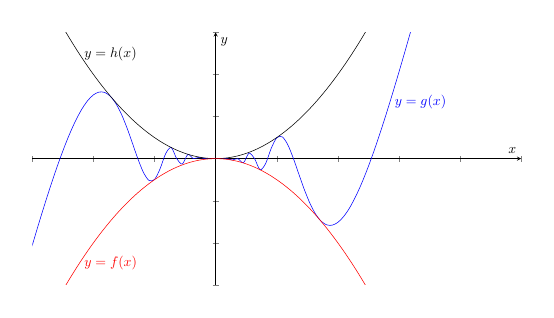
\begin{tikzpicture}[scale=0.5]
\begin{axis}[
 axis lines=middle,
 ticklabel style={fill=white},
 xmin=-1.5,xmax=2.5,
 ymin=-1.5,ymax=1.5,
 xlabel=$x$,ylabel=$y$,
 domain=-2:2.5,
 samples=100,
 smooth, 
 yticklabels={,,},
 xticklabels={,,},
 height=8cm,
 width=14cm]
\addplot[blue] {x*x*sin(4/\x r)}node[pos=0.65,anchor=west]{$y=g(x)$};
\addplot[black] { x*x}node[pos=0.25,anchor=west]{$y=h(x)$};
\addplot[red] {-x*x}node[pos=0.25,anchor=west]{$y=f(x)$};
\end{axis}
\end{tikzpicture}